\documentclass[12pt]{article}
\usepackage{geometry} % see geometry.pdf on how to lay out the page. There's lots.
\usepackage{natbib}
\usepackage{graphicx}
\usepackage{url}
\usepackage{color}
\geometry{a4paper} 

%%%%%%%%%%%%%%%%
%%%%%%%%%%%%%%


\title{Conversation, cognition and cultural evolution: \\a model of the cultural evolution of word order through pressures imposed from turn taking in conversation}
\author{Se\'{a}n G. Roberts and Stephen C. Levinson}
\date{} % delete this line to display the current date

%%% BEGIN DOCUMENT
\begin{document}
\maketitle

\section*{Abstract}

In conversation, speakers attempt to minimize the length gaps and overlaps between turns.  This imposes a pressure on processing which could have implications for the cultural evolution of structural properties of language.  We present an agent-based model of cultural evolution where agents take turns at talk in conversation.  When the start of planning for the next turn is constrained by the position of the verb the stable distribution of word orders evolves to match the actual distribution reasonably well.  We suggest that the interface of cognition and interaction should be a more central part of the story of language evolution.

\section{Introduction}

The evolution of linguistic structure is constrained by various cognitive pressures. For example, studies have argued that basic word order is adapted to pressures on efficient storage or processing \citep{hawkins1994performance,ferrer2008some} or the effectiveness of conveying semantic information \citep{goldin2008natural,schouwstra2014semantic}. 


%Cognitive pressures
%	Structures that are hard to process or produce will be avoided
%	(e.g. Hawkins 2004; Ferrer-i-Cancho, 2015)
%Conventional pressures
%	Linguistic structures are maintained and transmitted
%	(e.g. Dunn et al., 2011)
%Expressivity pressures
%	Structures which are easy to understand will be selected
%	(Goldin-Meadow et al., 2009; Schouwstra \& de Swart, 2014)
%
%But where do these pressures come from?


%http://faculty.wcas.northwestern.edu/matt-goldrick/blankensee-clarkgoldrickkonopka06.pdf

While these effects are part of the story, we suggest that the primary ecology of language is interaction - speakers taking turns in a conversation \citep{levinson2006human}.   The processing demands on comprehension and production are situated in, and largely dictated by, what is happening in conversation.  The way in which ideas and intentions are communicated is not through isolated signals, but in an interactional context.  Therefore, understanding the constraints and affordances of conversation is crucial for understanding the selective pressures on language use.    As Schegloff, one of the founders of the field of Conversation Analysis, put it: 

\begin{quote}
``What is the primordial natural environment of language use, within which the shape of linguistic structures such as grammar, have been shaped? Transparently, the natural environment of language is talk-in-interaction, and originally ordinary conversation.  The natural home environment of clauses and sentences is turns-at-talk.  Must we not understand the structures of grammar to be in some important respects adaptations to the turn-at-talk in a conversational turn-taking system with its interactional contingencies?'' \cite[p. 143-144]{schegloff1989reflections}
\end{quote}

In that article, Schegloff seems to mean that the biological capacity for using and acquiring language may have adapted to conversation.  While that is possible, here we focus on the implications for \emph{cultural evolution}.  The demands of interactive conversation should impose selective pressures on linguistic structures.  If there is variation in how effective different structures are in conversation, and if more effective structures are more likely to `replicate' and be used again, then this sets the scene for Darwinian evolution \cite{Croft_2000}.  


An example which links constraints from pragmatics to predictions about typology comes from Thompson's work on interrogatives (XXXX).  Thompson points out that interrogative structures make turn transition relevant (a question demands an answer), so in order to be effective, interrogatives should generally apply to prosodic units, and therefore appear at turn boundaries, rather than in the middle of turns.  This constraint leads to a specific prediction: languages that place the verb at the end of a sentence should have interrogative suffixes, not affixes.  We tested this statistically by looking at the probability of interrogative suffixes for different word orders in a sample of the world's languages, controlling for historical influence.  Indeed, we find that suffixes are much more likely than prefixes in verb-final languages (460 languages taken from \citealp{wals-26} and \citealp{wals-81}, mixed effects model controlling for language family, z = 3.92, p = 0.0001).  This is a well-known pattern in typology, but here we suggest that part of the pressure that lead to the emergence of the pattern could be motivated by pragmatics.


In this article, we consider a specific aspect of conversation - turn taking - and how it might impose a cognitive pressure which leads to the selection of specific grammatical structures in a cultural evolution framework.  While the work is preliminary, we hope to demonstrate the possibility of linking conversation, cognition and cultural evolution.

\subsection{A cognitive pressure derived from turn taking}

In a conversation, speakers take turns at talking and try to minimise the amount of gap or overlap between the turns \citep{sacks1974simplest}.  When talking in groups, there is competition for who speaks next \citep{levinson1983pragmatics}, and a delay in response is pragmatically marked, for instance, it can be interpreted as unwillingness \citep{Kendrick_Torreira_2015}.  This puts speakers under a pressure to respond quickly in conversation.  

Indeed, the average gap between questions and answers is around 200ms \citep{stivers2009universals}.  What makes this surprising is that the time to plan and begin executing a single word is at least 600ms \citep{indefrey2011spatial}.  That is, we must be anticipating what will happen as someone is speaking in order to start our own turn on time.  This imposes a kind of `crunch zone' in which production and comprehension happen at the same time (see figure \ref{fig:crunchZone}).

\begin{figure}[htbp]
\begin{center}
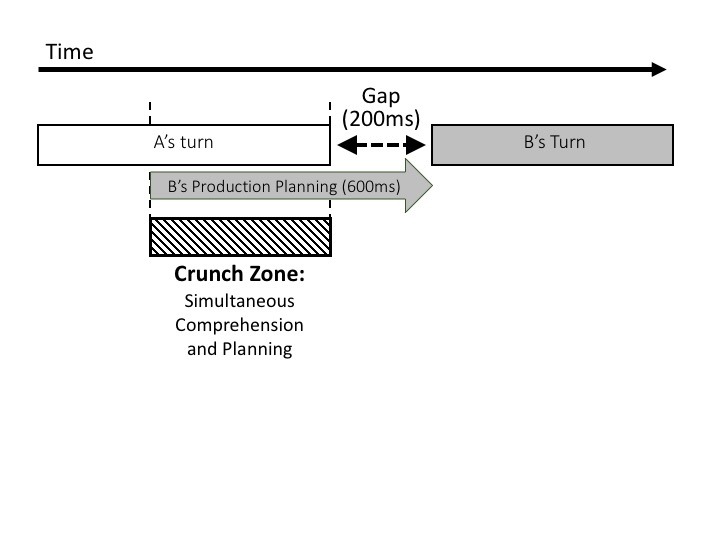
\includegraphics[width=\linewidth]{images/pdf/CrunchZone.pdf}
\caption{A schematic representation of turn taking.}
\label{fig:crunchZone}
\end{center}
\end{figure}

This is a harsh ecology for speech.  To put it in perspective, achieving this accuracy in timing is like standing 15m from a road and throwing a football into the window of a car that's passing at 35km/h.  There may be a large variety of adaptations, but we focus on basic word order as an illustration of how languages might adapt to the constraints of turn taking. 






\subsection{Linking processing and pragmatics}

If turn taking imposes cognitive pressures, then the structure of language should adapt. We should be able to see signs of these adaptations in today's languages.



%Patterns in linguistic structure are the result of a complex system of constraints from cognition and interaction

We could go further in linking pragmatics and typology by integrating constraints from online processing.  To see how this might work, take the following example.  In a typical utterance, the listener is given bits of information in sequence.  Figure \ref{fig:langExample} shows an example sentence from Portuguese.  Early in the sentence, we hear some crucial bits of information, for example the subject of the sentence and the topic, then the predicate (what's happening to the boy) and the syntactic frame.  Finally, we get the goal of the utterance.  However, a different structure could have been used.  For example, we could imagine a strange structure for Portuguese which provided morphological elements up front, like the subject of the prepositional phrase is female or that the verb is 3rd person and reflexive, and then got all the crucial bits of information at the end.  This is a terrible idea from a turn-taking perspective, because it puts all the crucial elements in the crunch zone, making it difficult for the next speaker to take their turn quickly.

\begin{figure}[htbp]
\begin{center}
\includegraphics[width=\linewidth]{images/pdf/LangExample.pdf}
\caption{An example of different possible structures of a sentence, and its implications for turn taking.}
\label{fig:langExample}
\end{center}
\end{figure}

Although this is a contrived example, in principle it suggests that turn taking has some implications for effective structures in language.  In other words, languages do not adapt just to our individual cognition, but to the way we use cognition in interaction.  If we had infinite time to prepare and process language, then these pressures would not apply.
However, the majority of language use happens in conversation, and in conversation we have to think fast.

Let us consider the implications for basic word order (the order of the subject, object and verb in a canonical transitive clause).  If the verb provides the syntactic frame for a sentence and is a crucial conveyor of the pragmatic action, then its position in the sentence might adapt to several pressures. Verbs in final position give speakers more time to plan the most complex component of the turn.  On the other hand, verbs in initial position allow the listener to interpret the previous turn and start planning their own turn earlier. 

At first, we might expect the best solution would be to keep important information away from the crunch zone (see figure \ref{fig:strategies}).  
However, turns exist in sequences.  In this case, the next turn would be very difficult for A:  They are trying to comprehend a crucial element in a crunch zone.  One solution is to co-ordinate structures.  If the crucial information is placed at the start of the turn, this means no crucial information is being provided at the crunch point.  That is, the constraints of turn taking provide a pressure for co-ordination of utterance structure.  

One problem with this solution is that B is planning crucial information during the crunch point.  Another solution might be to put the crucial information in the middle of the utterance.  This balances the distance from the crunch point for both comprehension and planning.
This has the added bonus of preserving crucial information from overlap.  A third solution might be to give maximum time for planning.  Having crucial information at the end of the turn means putting it in the crunch zone, but B can leave planning until later.  That is, they can start speaking without having planned the entire utterance.

In all cases, we see that the structure of A's turn has a knock-on effect on B's turn structure.  Any strategy can facilitate turn taking, as long as everyone is using the same strategy.

\begin{figure}[htbp]
\begin{center}
\includegraphics[width=\linewidth]{images/pdf/Tactics.pdf}
\caption{Different strategies to aid smooth turn taking.}
\label{fig:strategies}
\end{center}
\end{figure}

This could have implications for how languages change over historical time.
We would predict that a language would be more likely to change to facilitate better turn taking than in the opposite direction.  This suggests that the number of languages that facilitate turn taking should increase over time, while the number of languages that hinder turn taking should decrease.  

This could be tested in the following way.  First, we identify a constraint that turn taking makes on a particular linguistic structure.  That should lead to some predictions about the distribution of that structure we should see in the world's languages.  We can then test whether the prediction can be observed in real data.  

However, this involves two challenges.  First, the precise interactions between conversation, cognition and cultural evolution are not easy to predict, since they form a complex system.  In order to generate predictions, we implement a simple agent based model of turn taking.  Computational agents are simple computer programs whose behaviour we can specify.  By placing many agents together in a model, we can see how they interact.  In the sections below, we define and explore such an agent based model of cultural evolution through conversation.

The second challenge is testing whether the predictions from the model fit data in the real world.  This is also not straightforward because the distribution of linguistic structures in the world are complicated by historical factors.  In the next section, we explain this further and estimate the target phenomena which should emerge in the model.


%TANAKA
%Tanaka (2000, 2005)
%Canonical SOV order, incremental transformability: 
%Delayed projectability
%
%Perhaps we can expand the model again to model sentence final particles.
%Tanaka notes that the grammar of Japanese limits the projectability of turns.
%The predicate comes at the end of the sentence, and the sentence can be widely transformed by elements that come after the predicate.
%However, Kobin Kendric has suggested that they also potentially buffer transitions by giving extra time for B to respond.
%
%(10) [Tokyo 7, p.26] multiparty conversation; utterance-finals in bold
%
%In this example, we see that the sentence final particle is appearing constantly in overlap, suggesting that they work as elements that aid transition.

%
%Japanese has SOV order, which limits the projectability of turns (Tanaka, 2000, 2005)
%But sentence final particles might provide a `buffer'  (Kendrick)
%
%We would expect sentence final particles to be particularly helpful for verb-final languages, since they move the verb out of the crunch zone.
%Similarly, sentence initial particles would be helpful for verb initial languages, since they buffer planning of the crucial information.
%
%
%
%we noted that having a verb at the start of sentences is not optimal because B is planning a crucial piece of information in the crunch zone.
%One thing that might help this is if utterances had question initial phrases that could buffer the crucial information away from the crunch zone.
%
%Initial question phrases help to buffer planning
%Prediction: More helpful for V-initial languages
%Model:



\section{Identifying the target phenomenon}

We would like to account for two basic phenomena in word order patterns.  First, for the vast majority of language communities, speakers use the same basic word order for expressing the same kinds of meanings.  There is certainly optionality within languages, and individual variation.  For the most part, however, speakers do not use completely random word orders.  That is, basic word order is coordinated within a language community.

The second phenomenon is that some basic word orders are more frequent than others.  For example, if we count the raw number of basic word orders, then the pattern we see is that SOV and SVO more frequent that VSO order.  However, this does not take into account the historical relations between languages.  For example, many celtic languages are VSO, but they are all related historically, so it's unfair to count each as an independent point (see \citealp{Roberts_Winters_2013}).
  
In this study we will use Harald Hammarstrom's estimation of word order types in language isolates.  This also happens to be close to other estimates based on using non-isolates and controlling for historical relations.  This turns out to be 11\% VSO, 16\% SVO, 66\% SOV and other orders account for 7\%.  That is, the further from the start of the sentence the verb is, the more frequent that word order type.  The majority of the world's languages place the subject before the object in canonical transitive sentences, so we focus on those, but the model below does not actually distinguish between subjects and objects - only the position of the verb that is important.

In later sections, we also look at the interaction between basic word order and other typological variables.  In this case, we use data from the world atlas of language structures \citep{WALS2} in a mixed effects model.  This estimates the relationship between basic word order and other typological features when taking into account historical relations.  See the supporting information for details and results.


\section{A computational agent based model of turn taking}

We model a conversation as an interaction between two computational agents A and B.  Agent A produces a turn at talk which consists of  three abstract elements - a verb, a subject and an object.  There are three turn types - VSO, SVO and SOV.  The agents do not understand these elements, and there is no meaning associated with the elements.  This simply captures the idea that there's some linear order, with some elements being more crucial than others.

Each agent has an exemplar memory which stores all the turns it has heard.  When an agent produces a turn at talk, they select one turn from their memory at random to be the template for their utterance.  

Now agent B has to decide how to respond by choosing a template turn from their own memory.  However, we constrain the probability of choosing different turn types according to the distance between the verbs in the sequence.  For example, if A produces a VSO turn, then then B has more time to process this information and so is more likely to be able to produce a verb at the start of their sentence.  If A produces an SVO turn, then their verb is closer to the crunch zone and B is less able to produce a verb-initial turn.  If A produces a SOV turn, then the verb is in the crunch zone and so B is very unlikely to be able to produce a verb-initial sentence in time, and quite unlikely to be able to produce a verb-medial sentence in time.

To model this, each item in the agent's memory is given a weight which affects its probability of being chosen.  If A produces a turn $T_1$ which has the verb at position $V_1$ (start = 0, middle = 1, end = 2) and a length $L_1$ (at this stage, all turns have a length of 3), then a responding turn by B, $T_2$, which has the verb at position $V_2$ is given the following weight:

\begin{equation}
W_{T_2} = ((L_1 - V_1) + V_2) ^ \alpha
\end{equation}

Where $\alpha$ is a parameter which controls the strength of the effect.  When $\alpha = 1$, then the weight increases linearly as the distance between the two verbs increases.  The probability of choosing item $i$ from a memory which contains $M$ items is then directly proportional to its weight.

\begin{equation}
P_i = \frac{W_i}{\sum_{x=1}^{M} W_x}
\end{equation}

Put another way, agents are less likely to choose turn structures which involve more verb processing in the crunch zone.  The $\alpha$ parameter, then, controls how quickly the processing cost increases with time.  This mechanism captures the basic idea that the location of crucial information in A's utterance has a knock-on effect for the structure of B's turn.  The constraint on B's choices are greatest when A produces a turn with the verb at the end.

Conversations proceed in the following way.  A produces a first turn by selecting randomly from their memory.  B then produces a turn, drawing from their memory according to the weight function above.  Then A produces a third turn, weighting their selection by the turn type that B produced.  Then B responds, and so on.  

Conversations are independent from each other, and always start with an unweighted selection.  Therefore, we can manipulate the strength of the effect from turn taking.  For example, agents can have one conversation of three turns, which imposes a constraint after each turn, or three conversations of a single turn, in which case the turn taking constraints have no effect.  The greater the number of turns in a conversation, the greater the knock-on effect of the crunch zone.  In each generation (see below), agents will have $N_{conversation}$ conversations with $N_{turn}$ turns each.

We also model a small amount of noise in communication.  With a small probability $\beta$ (noise), an agent produces a random turn type from all possible turn types.

\subsection{Cultural evolution}

Now we need a model of cultural evolution.  We start with a small population of $N_{agents}$ `adult' agents.  Each agent is initialised with a random selection of turn types in their memory.  This means that populations are initialised with no bias in their word order preferences.  Each agent is randomly paired with another agent and they have a conversation with $N_{turn}$ turns.  This repeats until they have had $N_{conversation}$ conversations.  This results in a series of turns and conversations, and we can measure the frequency of each turn structure.

At the same time, there is a second population of `child' agents listening to the conversations of the adult population and `learning' from them by adding their turn structures to their exemplar memory.
That is, generation 2 are like children acquiring language.  When the adult generation are done with their conversations, they are removed from the population and the child generation `grows up' and become adults.  This new generation starts having conversations in the same way as the first generation, while a new child generation (generation 3) listen and learn.

This repeats for $N_{generation}$ generations.  For each generation, we can track how the proportions of each type of sentence change.

\subsection{Sentence particles}

We can expand the model again to explore the role of sentence final particles.  
Tanaka (2000;2005)\nocite{tanaka2000turn,tanaka2005grammar} notes that the grammar of Japanese limits the projectability of turns.   The predicate comes at the end of the sentence, and the sentence can be widely transformed by elements that come after the predicate.  This appears to work against rapid turn taking.  However, sentence final particles can potentially act as a `buffer' which push crucial information away from the crunch zone and allow more time for the next speaker to plan their turn (this insight from Kobin Kendrick, personal communication, see figure \ref{fig:Particles}).  

\begin{figure}[htbp]
\begin{center}
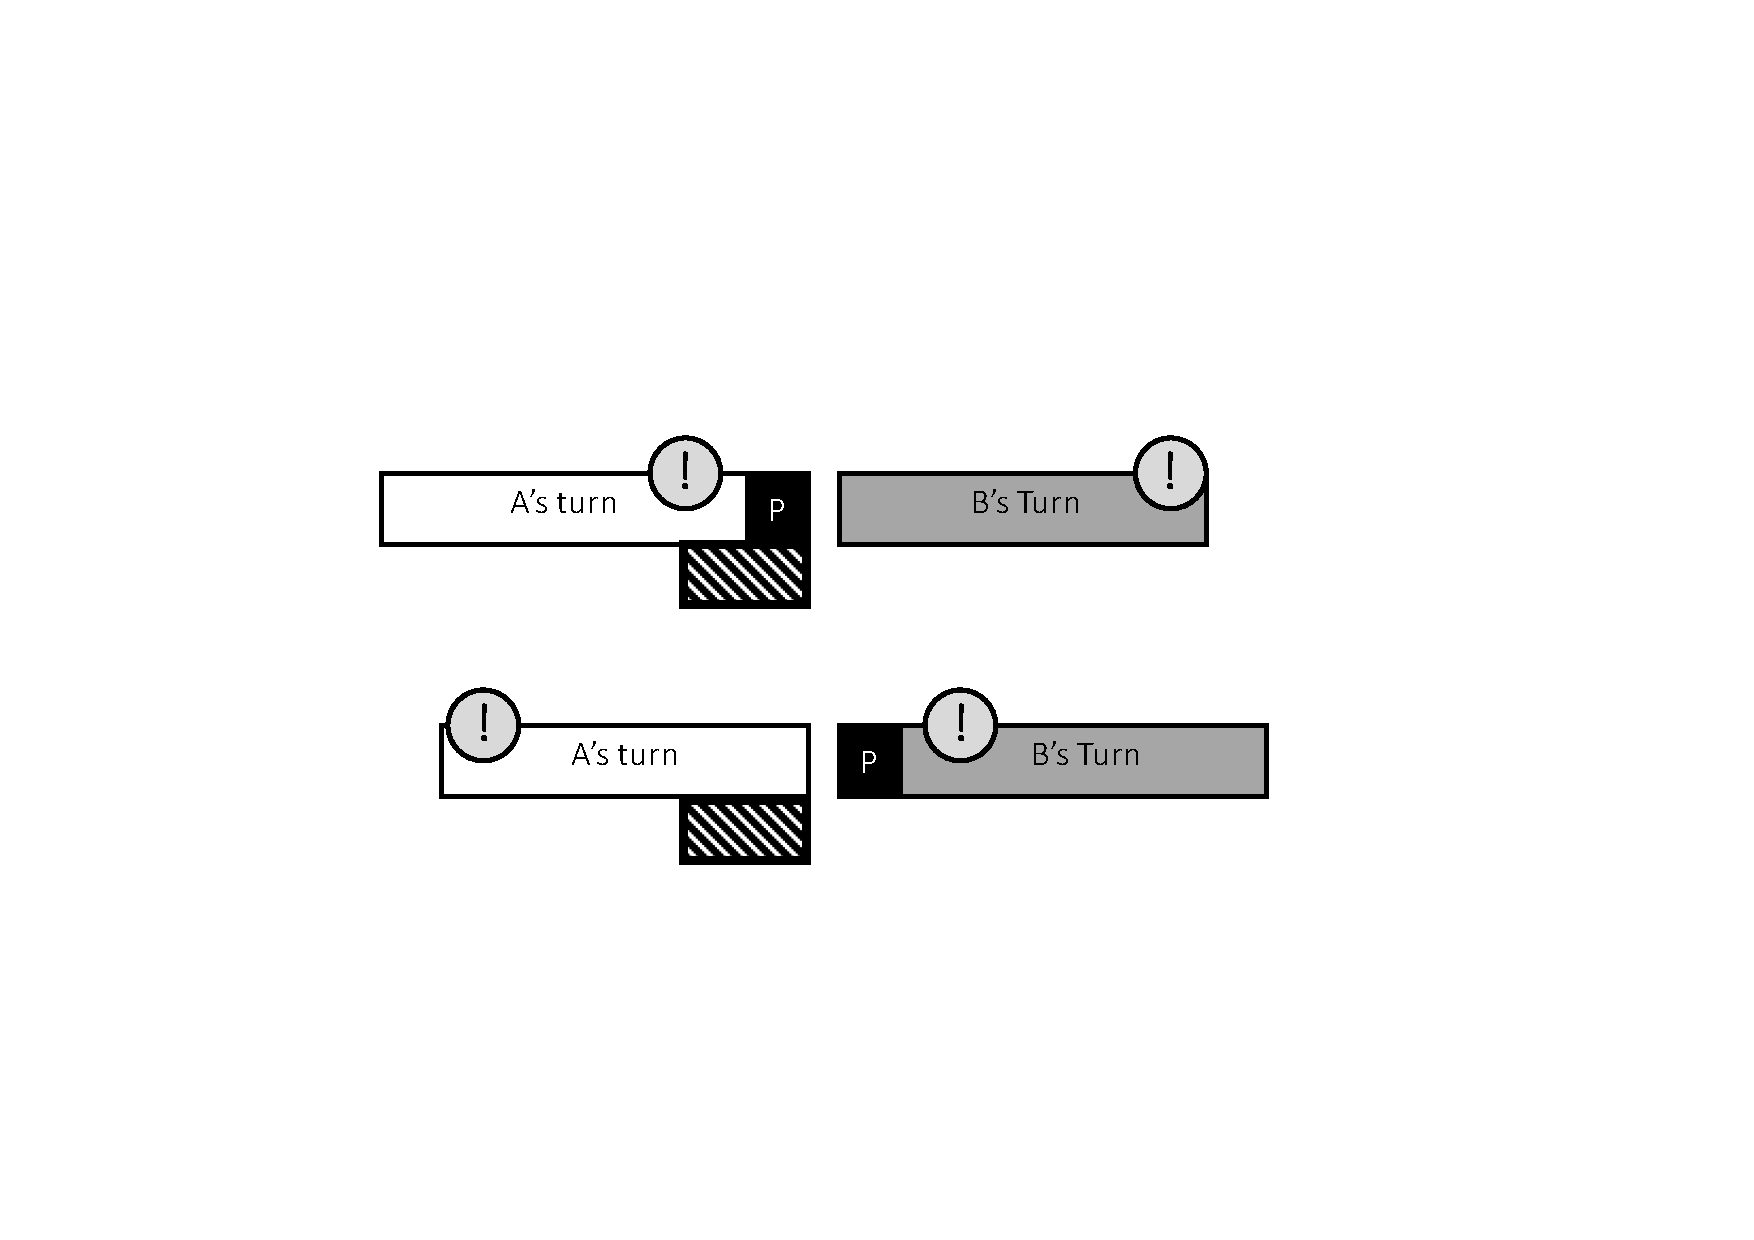
\includegraphics[width=100mm]{images/pdf/Particles.pdf}
\caption{Sentence particles `P' can act as a `buffer' between turns, taking the crucial information away from the crunch zone.}
\label{fig:Particles}
\end{center}
\end{figure}


In example of Japanese conversation in figure \ref{fig:Tanaka}, we see that the sentence final particle is appearing constantly in overlap.  This suggests that they can be treated as non-crucial elements of the turn (the overlap in the example can be partly attributed to the general projectability of the sentence in which the two speakers are agreeing with each other, but in general particles are not overlapped).  A theory based on ease of production or perception which does not consider relationships between turns would have a hard time explaining why speakers bother to include these.  

\begin{figure}[htbp]
\begin{center}
\includegraphics[width=\linewidth]{images/pdf/TanakaExample.pdf}
\caption{A conversation in Japanese.  Square brackets indicate where the next speaker overlaps with the previous one.  The utterance final particles are in bold. Adapted from \cite{tanaka2000turn}, Tokyo 7, p.26.}
\label{fig:Tanaka}
\end{center}
\end{figure}

In this case, turn final particles aid transition of this verb-final language.  However, the general prediction about which word order would benefit from final or initial particles is difficult to make.  If a language is verb-initial, should sentence particles come at the start of the turn, or the end of the previous turn?  Both would be logically helpful, but which are more likely to emerge?  Are there some word orders which are less likely to need particles at all?  It is difficult to work out the logical implications in a cultural evolutionary system, but this is precisely what the model is for.  We can use it as a kind of transparent thought experiment.

%The first alternative model included initial question particles.  As well as the three basic word orders, agents could produce versions with initial question particles (6 types to choose from).  There was an extra production cost for structures with a question particle, but possibly a lower responding cost, since the question particle acted as a buffer, increasing the distance between verbs.

Sentence particles were included in the model as follows.  As well as the three basic word order types, agents could also produce versions with a sentence final or sentence initial particle (9 types to choose from).  Turn types with particles were less likely to be picked for production, since they are slightly longer (agents prefer to produce shorter turns).  The relative length of particles to other words (verb, subject and object) could be manipulated via a parameter $p$.  From the examples in Japanese, we would expect particles to be shorter than most words.  The inclusion of a particle which added distance between verbs in a turn boosted the possibility that the verb can come earlier in a following sentence.  

\subsection{Summary of assumptions}

Here we summarise the basic assumptions of the model:

\begin{itemize}
\item All turns contain verbs
\item We do not model semantics or detailed syntax/morphology
\item Speakers must minimise gaps and overlaps
\item Planning crucial elements is increasingly difficult as it approaches the `crunch zone'
\item Verbs are crucial elements (they are hard to plan)
\item The production cost of sentence is related to sentence length 
(though in the main model all sentences have the same length)
\item  In cultural evolution, agents learn by observing others and storing examples of behaviour
\item Generations are discrete
\end{itemize}

Clearly, these assumptions are idealisations, and language is more complex that this.  Even the assumption that all turns contain verbs is clearly wrong when looking at ordinary conversation.  However, as a starting point, we think that this is reasonable.  We are attempting to construct the simplest model which will help us think about the relationships between conversation, cognition and cultural evolution.  One way to think about the model is that it is modelling only some conversations, not every interaction between agents, and that the selective pressure only applies in turns which match the conditions above.

\section{Results}

Figure \ref{fig:SingleRuns} shows three independent runs of the model with a population of 10 agents taking 2 conversations of 10 turns each (noise level $\beta$ = 0.01).  Along the horizontal axis we see generations and each line represents how the frequency of each type of sentence changes over time.  We see that in the first generation, agents are equally likely to use any of the three types, but that the use of VSO rapidly declines.  In the first two runs, both SVO and SOV are used for some time, but after about 15 generations, all agents are using SOV all the time (with some small deviations due to noise).  So, we can classify the language of these agents as SOV.  In the third run, enough agents selected SVO by chance that the conventional pressure pushed the frequency up.  Eventually, the third population converges on SVO order.  

\begin{figure}[htbp]
\begin{center}
\includegraphics[width=\linewidth]{images/pdf/SingleRuns.pdf}
\caption{Proportions of each turn type used at each generation for three independent runs of the main model.}
\label{fig:SingleRuns}
\end{center}
\end{figure}

We ran the model 1000 times measured the proportion of runs that converge to each word order type.  In every simulation, the population converged on a single word order type within 100 generations.   Figure \ref{fig:MainModelResults} shows the results ($\alpha$ = 0.1).  When agents only have conversations with 1 turn (no constraints from turn taking), then each word order type is equally likely to win.  When turns follow each other within a conversation, the proportions look qualitatively like the actual distribution of word orders we see in real languages:  SOV is most frequent followed by SVO and VSO.



\begin{figure}[htbp]
\begin{center}
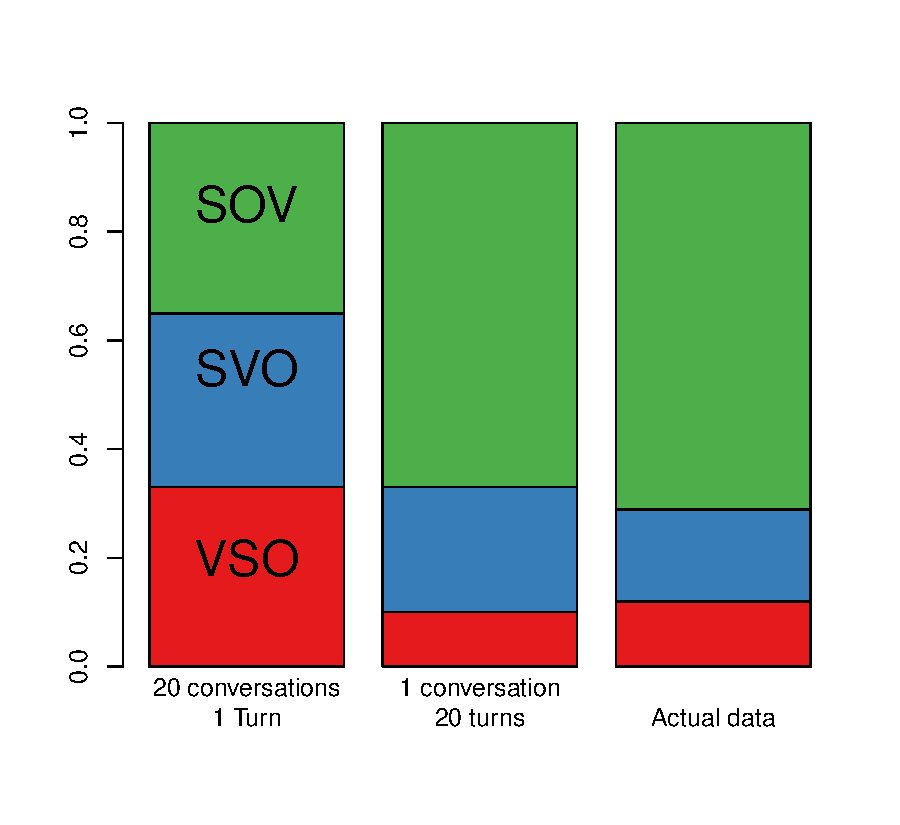
\includegraphics[width=\linewidth]{images/pdf/MainModelRes.pdf}
\caption{Proportions of each turn type that 1000 generations converge to in:  a model without pressures for turn taking (left); a model with turn taking constraints (middle); and actual language data (right).}
\label{fig:MainModelResults}
\end{center}
\end{figure}

Essentially, the turn taking constraints impose a bias for pushing the verb out of the crunch zone to the end of the sentence.  However, one crucial result is that although there is a small proportion of populations with VSO order, within those populations \emph{all} agents are using VSO order.  That is, the model is producing the two target phenomena: convergence within populations and a bias for verb-later orders between populations.

The results in figure \ref{fig:MainModelResults} fit the data qualitatively, but also quantitatively (the proportions as well as the ranks are quite close to the real ones).  The quantitative fit depends on the parameters of the model.  Figure \ref{fig:Alpha} shows how the distribution of word order types varies with the $\alpha$ parameter, which controls how the distance between verbs relates to the processing cost.  When $\alpha$ is close to 0, there is little difference between each of the sentence types in any context, and roughly the same proportion of each sentence type emerges.  When $\alpha$ is positive, reflecting greater processing cost as the verbs enter the crunch zone, then the SOV advantage appears.  If processing cost scales linearly ($\alpha$ = 1), then the model predicts that almost all languages should show SOV order.  With negative values of $\alpha$, where cost \emph{decreases} as the verb enters the crunch zone, we see a preference for VSO languages.  This suggests that the best fitting assumption would be for a positive, convex function: the cost is large for verbs inside the crunch zone, but rapidly declines as the verb moves further away.  

\begin{figure}[htbp]
\begin{center}
\includegraphics[width=\linewidth]{images/pdf/AlphaSettings.pdf}
\caption{Right: how the function which relates the distance between verbs in neighbouring turns and processing cost with the $\alpha$ parameter.  Left: how the proportions of different word order types varies with the $\alpha$ parameter.}
\label{fig:Alpha}
\end{center}
\end{figure}


The supporting information shows that the model results are robust to settings of various parameters, including $N_{agents}$, $N_{conversation}$, $N_{turns}$ and $\beta$.


%\subsection{Initial question particles}
%
%Figure \ref{fig:QParticles} shows the results for a model including question particles ($N_{agents} = 10$, $\alpha$ = 0.1, $\beta$ = 0.05).   Without the turn taking constraints (20 conversations of 1 turn each), the model predicts that no language should have initial interrogative phrases.  This is because there's an extra production cost associated with the question particle.  However, with the constraints from turn taking, we see that initial question phrases are more likely for verb initial languages.  We see a qualitatively similar pattern in the real data.
%
%\begin{figure}[htbp]
%\begin{center}
%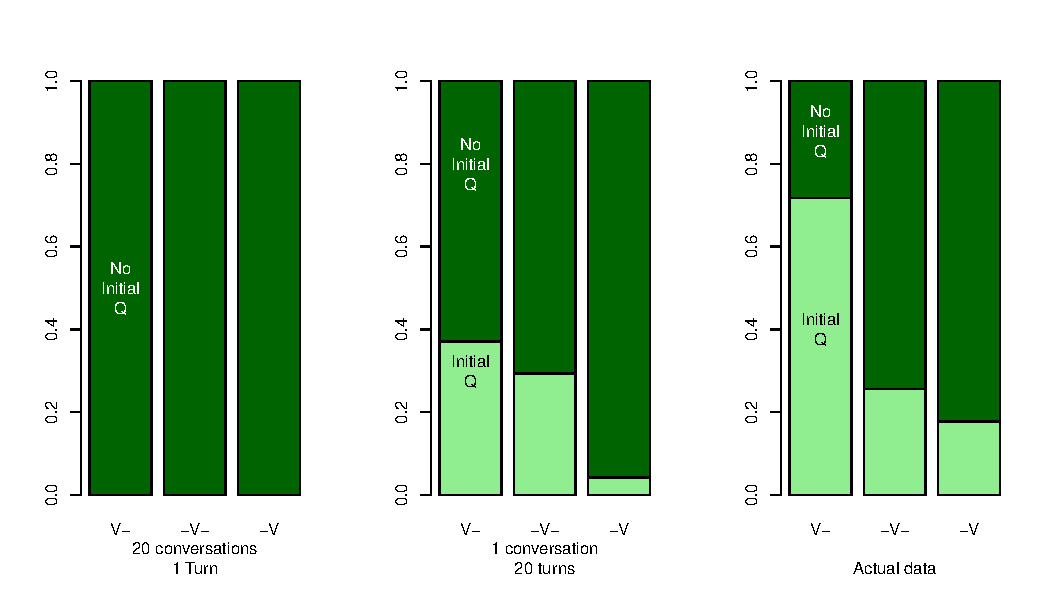
\includegraphics[width=\linewidth]{images/pdf/QParticle.pdf}
%\caption{Distribution of word order types and the presence of absence of an initial question particle.}
%\label{fig:QParticles}
%\end{center}
%\end{figure}


\subsection{Sentence final particles}

Figure \ref{fig:SParticles} shows some results for sentence final particles ($\alpha$ = 0.1, $\beta$ = 0, $p$ = 0.5, $N_{agents}$ = 10, comparing 20 conversations of 1 turn with 10 conversations of 2 turns).  The model without turn taking constraints predicts that languages are similarly likely to have initial or final sentences regardless of verb position.  However, with the constraint we see two things: Initial particles are more likely than final particles for verb initial languages, and that, for verb final languages, final particles are proportionately more likely. That is, if a language happens to settle on verb final structures, it is also more likely to develop sentence final particles.  This prediction also matches the real data quite well (data from position of polar question particles, \citealp{wals-92}, see SI).  Interestingly, it also predicts that verb final languages should be less likely to have particles at all.

\begin{figure}[htbp]
\begin{center}
\includegraphics[width=\linewidth]{images/pdf/SentenceFinalParticles.pdf}
\caption{Distribution of word order types and the presence of absence of sentence particles, with no turn taking constraints (left), with turn taking constraints (middle) and derived from real language data (right)}
\label{fig:SParticles}
\end{center}
\end{figure}

However, this result was not robust to changes in parameters.  The fit to the data was better when noise level was low and the inclusion of a question particle in a buffer zone had a big effect.  This is a reasonable assumption, given that the first model predicted that the processing cost declines rapidly as the verb moves away from the crunch zone.  Outside of a narrow window around the parameters above, the predictions range from no effect to the opposite of the effect we see in the data (final particles more likely for verb-final languages).  This suggests that the phenomenon emerges only under specific conditions.    


\section{Discussion}

In this article, we suggested that turn taking in conversation imposes constraints on the information structure of turns.  Languages should adapt to these constraints, and we should see evidence of this adaptation in the structures of the world's languages.  Support for this idea can be found by identifying a constraint that conversation imposes, generating a prediction about the distribution of linguistic structures that should emerge from these constraints, and then testing this prediction against real data.  We suggested that the need for rapid turn taking imposes a `crunch zone' for online language processing around the ends of turns, and hypothesised that this might affect the optimal position of crucial elements in a clause.  We presented an agent based model to help generate predictions about how these constraints should affect the cultural evolution of language, then compared the results to real data.  We found a reasonable qualitative match between the output of the model and the distribution of basic word orders in the real world.

The model suggests that speakers within a culture will co-ordinate their grammatical structures, and that any of the basic orders can become the conventional way of communicating.  However, because the structure of a prior turn has knock-on effects for the production of the next turn, there is a bias for cultures to evolve towards pushing the verb further back in the turn.  This leads to a distribution of basic word order which mirrors the distribution we see in the real world.

There are many issues to resolve.  The model is extremely simple and makes many assumptions that could be relaxed.  The parameters also need to be tied to specific cognitive mechanisms, rather than abstract notions of processing cost.  Rules of the sequential organisation of conversation could be built into the model.  The model also makes more general predictions about grammatical structures within conversations which could be tested.  For example, do speakers alter the information structure of their turns to aid processing through by local co-ordination?  However, it serves as a useful tool for thinking about the relationship between conversation and cognition in a cultural evolution framework.  



\bibliographystyle{apalike}
\bibliography{/Users/sgroberts/Documents/PhD/Biblography}

\end{document}